\documentclass[10pt]{beamer}

\mode<presentation> 
{
  \usetheme{Diku}
  \beamertemplatenavigationsymbolsempty
  \setbeamercovered{invisible}
%  \setbeamercovered{transparent}
}


% { \usetheme[nat,dogma]{Frederiksberg} }
%{ \usetheme[nat]{Frederiksberg} }

% \usepackage[danish]{babel}
\usepackage[latin1]{inputenc}
\usepackage{times,pslatex}
\usepackage[T1]{fontenc}
\usepackage[english]{babel}
\usepackage{hyperref}

\usepackage{multimedia}
\usepackage{francois-preamble}
\usepackage{multirow}
% \usepackage{multimedia}


\newcommand{\cc}{{c\!\!,}}
\newcommand{\degr}[1]{{{#1}^\circ}}
\DeclareMathOperator{\idf}{idf}

\title{Content Based Image Retrieval}

\author[S. Olsen] % (optional, use only with lots of authors)
{S�ren I. Olsen}
% Copied from Francois Lauze

\institute[DIKU] % (optional, but mostly needed)
{
  Department of Computer Science\\
  University of Copenhagen
}

\date[2014 B2] % (optional, should be abbreviation of conference name)
% {Research Presentation, Diku 2006}

% Insert page numbers
\pagenumbering{arabic}
\setbeamertemplate{footline}{\hspace{5pt}\insertpagenumber\vspace{10pt}}

\definecolor{gold}{rgb}{0.95,0.83,0.0}
\definecolor{orange}{rgb}{0.95,0.7,0.0}
% \definecolor{backblue}{rgb}{0.93,0.94,0.99}
\definecolor{backblue}{rgb}{0.95,0.94,0.99}
\setbeamercolor*{background canvas}{bg=backblue} 



\newcommand{\myemph}[1]{{\color{blue}{#1}}}
\newcommand{\intrg}[1]{\int_{{#1}=-\infty}^\infty}
\newcommand{\intRR}{\int_{-\infty}^\infty}

\AtBeginSection[]
{
  \begin{frame}<beamer>{Outline}
    \tableofcontents[currentsection,currentsubsection]
  \end{frame}
}


\begin{document}
\maketitle

% would be cool with more images showing applications


%-------------------------------------------------------------------
%   Start slides
%-------------------------------------------------------------------

\begin{frame}
  \frametitle{Plan for today}
  \begin{itemize}
  \item How to query Image Databases \\[3mm]
  \item The idea of visual words, codebook, bag of visual words. \\[3mm]
  \item The two main ingredients for building visual words are image
    descriptors and data clustering.
  \end{itemize}
\end{frame}


% \section{Introduction}

%-------------------------------------------------------------------
\begin{frame}
  \frametitle{Querying Images}
  \begin{itemize}
    \item Example from Google Images: Query using the word \texttt{apple}
    \begin{center}
      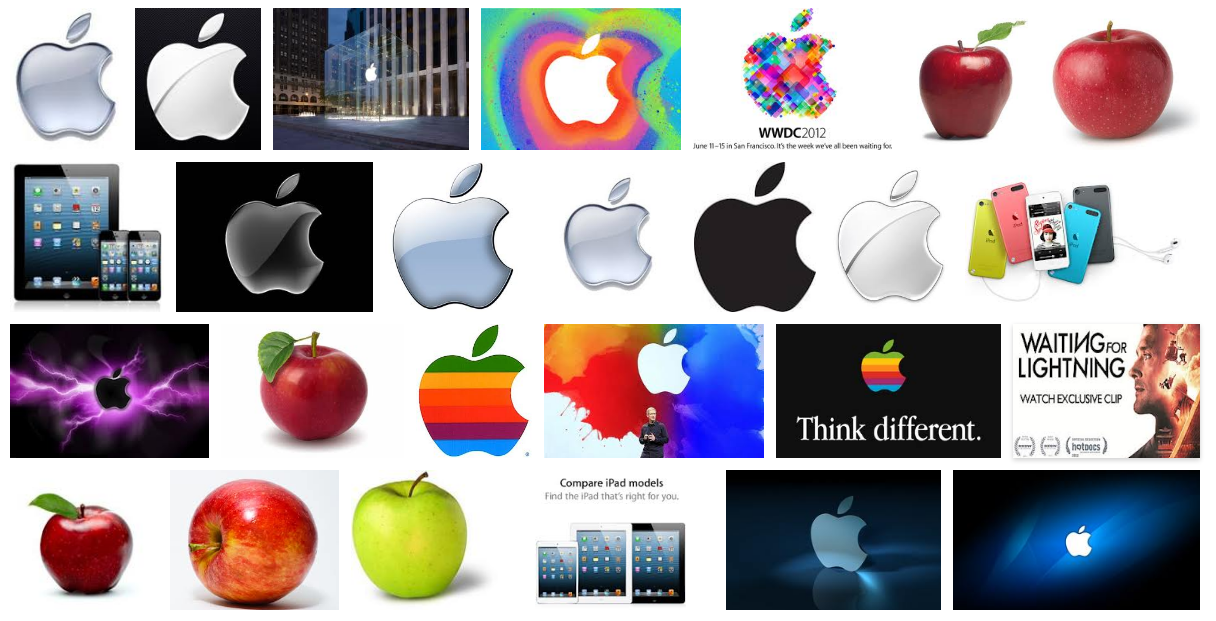
\includegraphics[width=0.8\textwidth]{FIGURE/GoogleAppleQuery}
    \end{center}
  \item Maybe not what expected! Try yourself and observe difference
    when using \texttt{apple} and \texttt{an apple}
  \end{itemize}
\end{frame}


%-------------------------------------------------------------------
\begin{frame}
  \begin{itemize}
  \item Simple textual description may fail. Reasons are multiple:\\[3mm]
    \begin{itemize}
    \item Language ambiguity ... \\[3mm]
    \item  Lack of proper image annotation ... \\[3mm]
    \item {\color{red}{Can you think of others?}}
    % Something hard to describe in few words - a story
    % Something hidden in the image composition - something missing
    \end{itemize}
  \end{itemize}
\end{frame}


%-------------------------------------------------------------------
\begin{frame}
  \frametitle{Another approach}
  \begin{itemize}
  \item Replace simple textual description by content based analysis.  \\[5mm]
  \item {\color{red}{\bf Exercise:} What content?} \\
           Discuss for 1 minutes with your neighbor what might be good
           image features for CBIR \\[5mm]
  \pause
  \item Use for instance Intensity, color, texture, shape etc... in a
    global or local setting.
%   \item Find efficient ways to answer the question:\\
%     \emph{What makes an image of an apple resemble an image of an apple?}
  \end{itemize}
\end{frame}


%-------------------------------------------------------------------
\begin{frame}
  \frametitle{An Inspiration: Text Mining}
  \begin{center}
    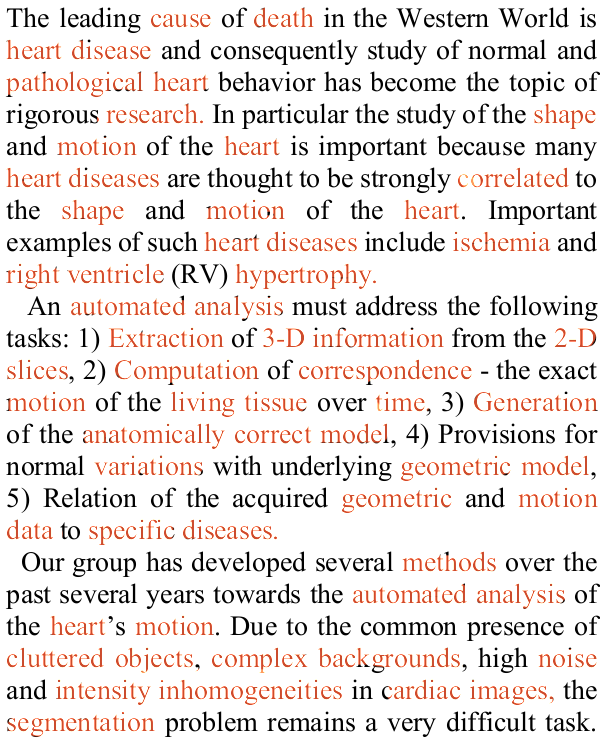
\includegraphics[width=0.5\textwidth,height=0.8\textheight]{FIGURE/ScreenshotMETAXAS}
      ~~
    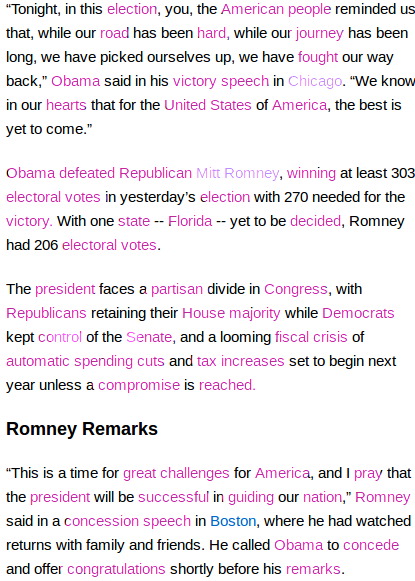
\includegraphics[width=0.5\textwidth,height=0.8\textheight]{FIGURE/ScreenshotBloomberg}
  \end{center}
\end{frame}


%-------------------------------------------------------------------
\begin{frame}
  \frametitle{Some statistics from these documents}
  Partial word count of the most frequent ones, eliminating very common ``the, and, of, is \dots''
  \vspace{-3mm}
  \begin{columns}
    \column{0.5\textwidth}
    \begin{center}
      Document 1
    \end{center}
    \vspace{-5mm}
    \begin{itemize}
    \item 7 times \textbf{heart}
    \item 4 times \textbf{disease(s)}
    \item 3 times \textbf{motion}
    \item 2 times \textbf{geometric}
    \item 2 times \textbf{shape}
    \item 2 times \textbf{model}
    \end{itemize}
    \column{0.5\textwidth}
    \begin{center}
      Document 2
    \end{center} 
    \vspace{-5mm}
    \begin{itemize}
    \item 3 times \textbf{elect(ion|oral)}
    \item 2 times \textbf{America(n)}
    \item 2 times \textbf{president}
    \item 2 times \textbf{speech}
    \item 2 times \textbf{state(s)}
    \item 1 time \textbf{heart}
    \end{itemize}
  \end{columns}
  ~\\
  \begin{itemize}
  \item Even discarding  grammatical structure, very different distributions.
  \item Some variation around a word were grouped ``disease|diseases'', ``election|electoral'', ``America|American''...
  \end{itemize}
\end{frame}


% \section{Bag of Visual Words}
% \label{sec:bovw}


%-------------------------------------------------------------------
\begin{frame}
  \frametitle{Visual Words}
  \begin{itemize}
  \item Visual words: what to choose?
    \begin{center}
      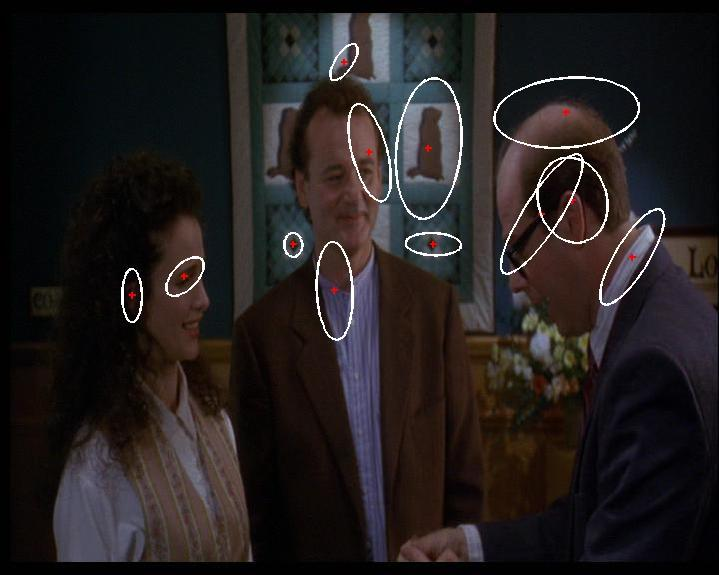
\includegraphics[width=0.5\textwidth]{FIGURE/groundhogday}~~
      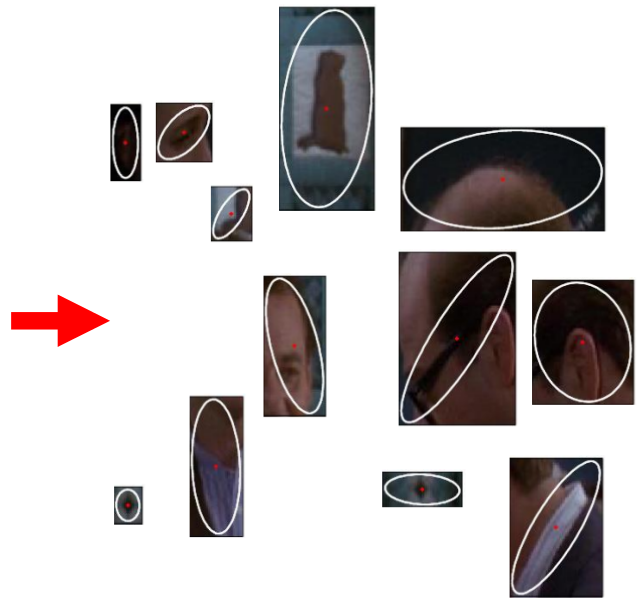
\includegraphics[width=0.5\textwidth]{FIGURE/gdwords}
    \end{center}
  \item Here patches centered around Harris Interest points.
  \item Other possibilities. Here we use SIFT descriptor (more than
    16000 citations means it must be interesting)
  \end{itemize}
\end{frame}


%-------------------------------------------------------------------
\begin{frame}
  \frametitle{Visual Words}
    \begin{itemize}
  \item Choose output from SIFT as building blocks for visual words.
  \item Produces generally 1000 -- 100.000 features per image. \\
    \begin{center}
      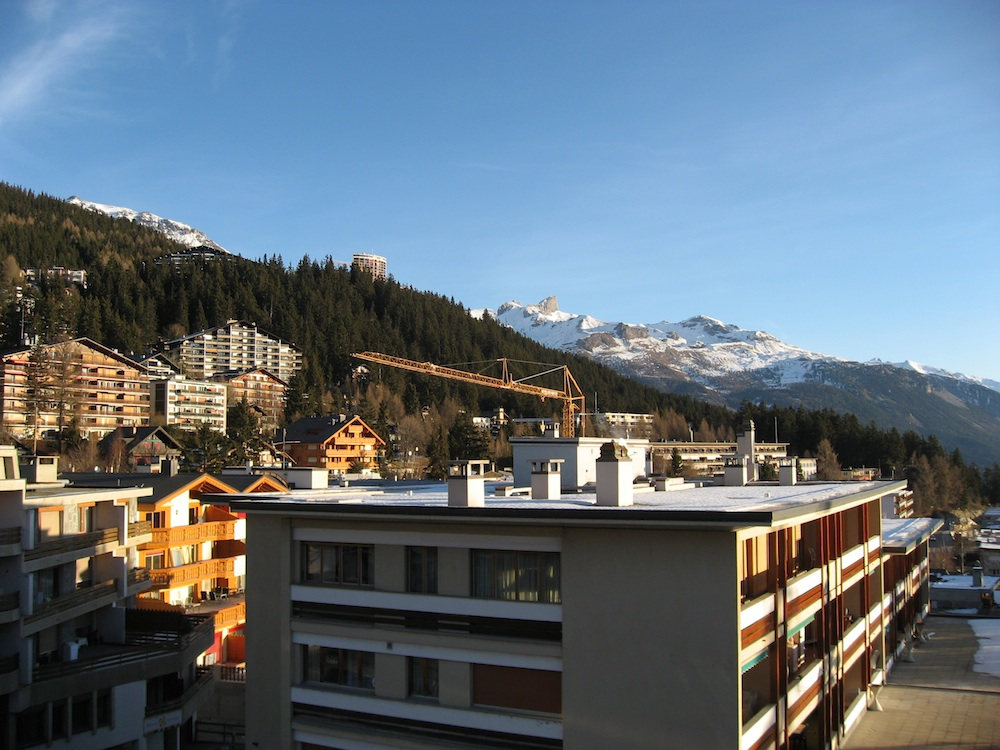
\includegraphics[width=0.5\textwidth]{FIGURE/crans_1_small}~~
      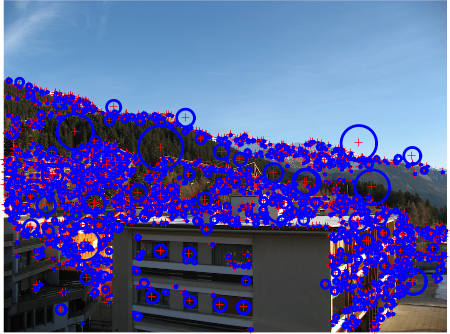
\includegraphics[width=0.5\textwidth]{FIGURE/cranswithsift} \\[2mm]
    \end{center}
  \item Some are similar in content (as for text, e.g., ``Election / Electoral'')
  \item So group them by similarity.
  \end{itemize}
\end{frame}


%-------------------------------------------------------------------
\begin{frame}
\frametitle{What and how to sample}
  \begin{itemize}
  \item Points sampled in a grid
  \item Points detected as Blobs, Corners, Centers of symmetri, ...
  \item Areas: Segments, Objects (what is that?) \\[5mm]
  \end{itemize}

Which descriptors are best (most discriminative, yet robust/general)?
  \begin{itemize}
  \item Histograms of color, textons (texture elements) ?
  \item Coded spatial layout (eg. SIFT-like) ?
  \item ...
  \end{itemize}
\end{frame}


%-------------------------------------------------------------------
\begin{frame}
\frametitle{MPEG 7}
  \begin{itemize}
  \item Is a Multimedia Content Description Interface Standard \\[3mm]
  \item Defines a set of image and video descriptors including color
    descriptors, shape descriptors, motion descriptors etc. \\[3mm]
  \item Includes language for specifying the relations between
    descriptors and their spatial (or other) relationships. \\[3mm]
  \item Try Google {\color{blue}{MPEG 7 Standards}}. \\[3mm]
  \item There is much more to the story than you will learn here.
  \end{itemize}
\end{frame}





%-------------------------------------------------------------------
\begin{frame}
\frametitle{Colors}

Humans register electromagnetic radiance with a vawelength 
$\lambda$ between 400 nm and 700 nm as colored light.

$$
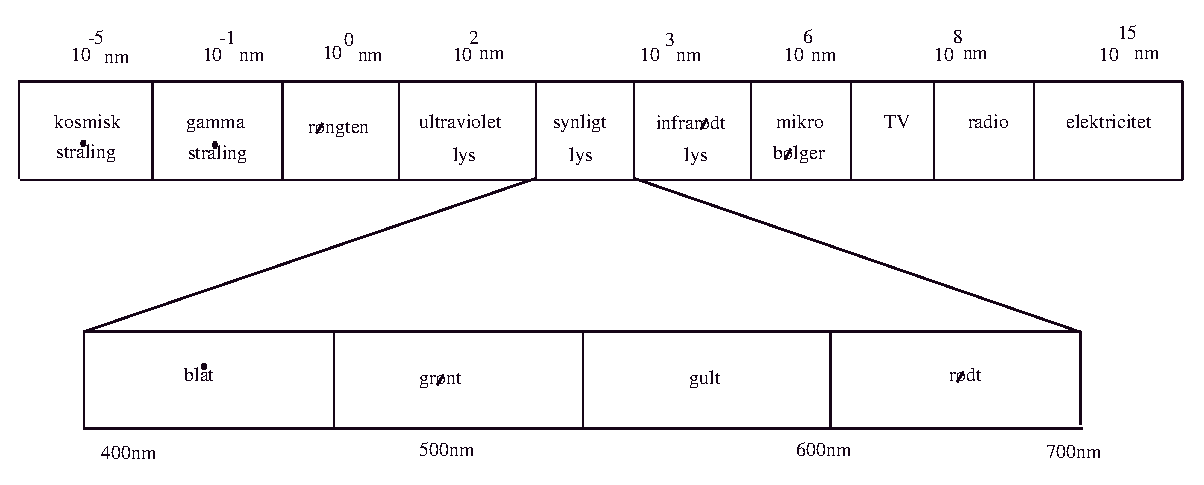
\includegraphics[width=8.0cm]{FIGURE/elektro.eps}
$$
\end{frame}


%-------------------------------------------------------------------
\begin{frame}
By using 3 sensors, sensitive to vawes in the red, the green and the blue 
area it is possible to represent a subset of the possible colors as an
RGB-value.\\[3mm] 

\begin{center}
\begin{tabular}{l r}
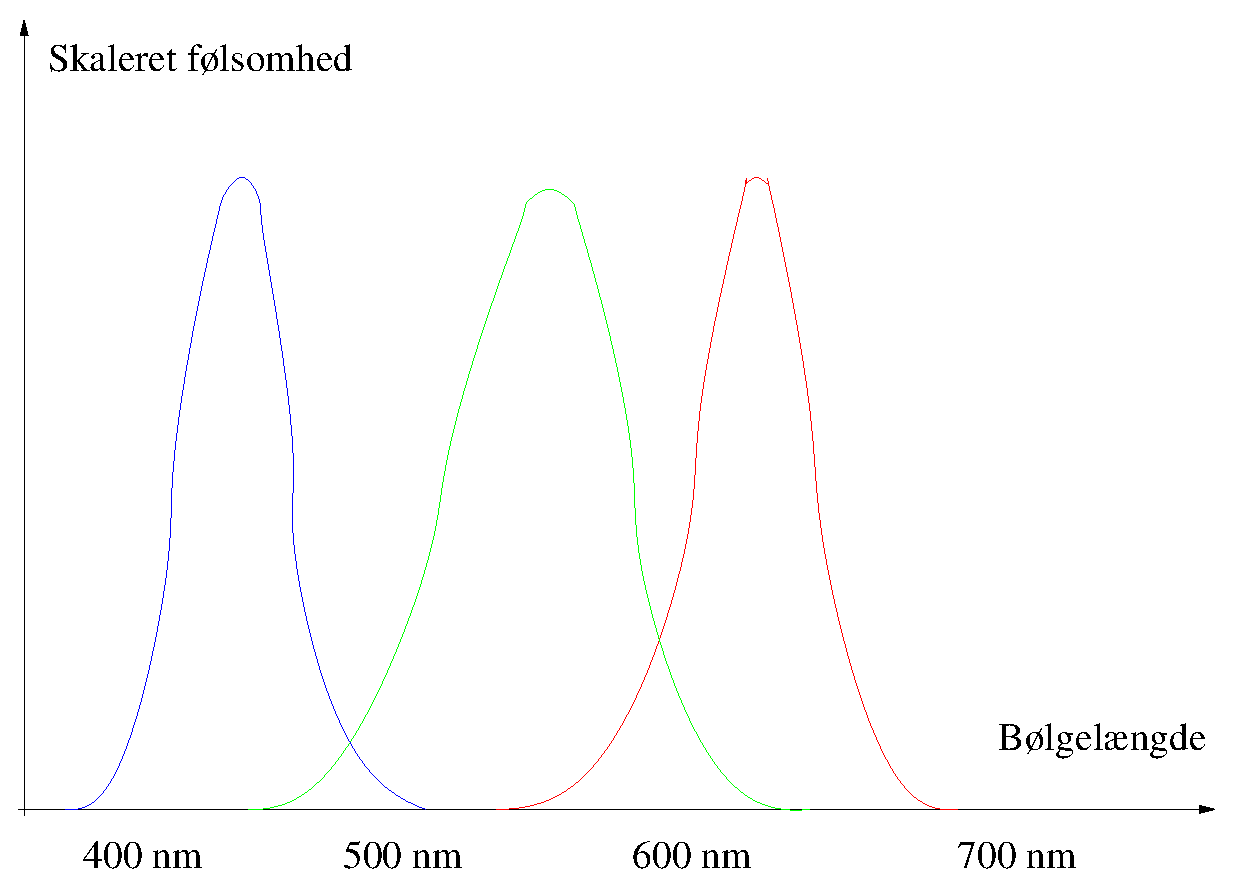
\includegraphics[width=4.5cm]{FIGURE/spectralfilters.eps}
&
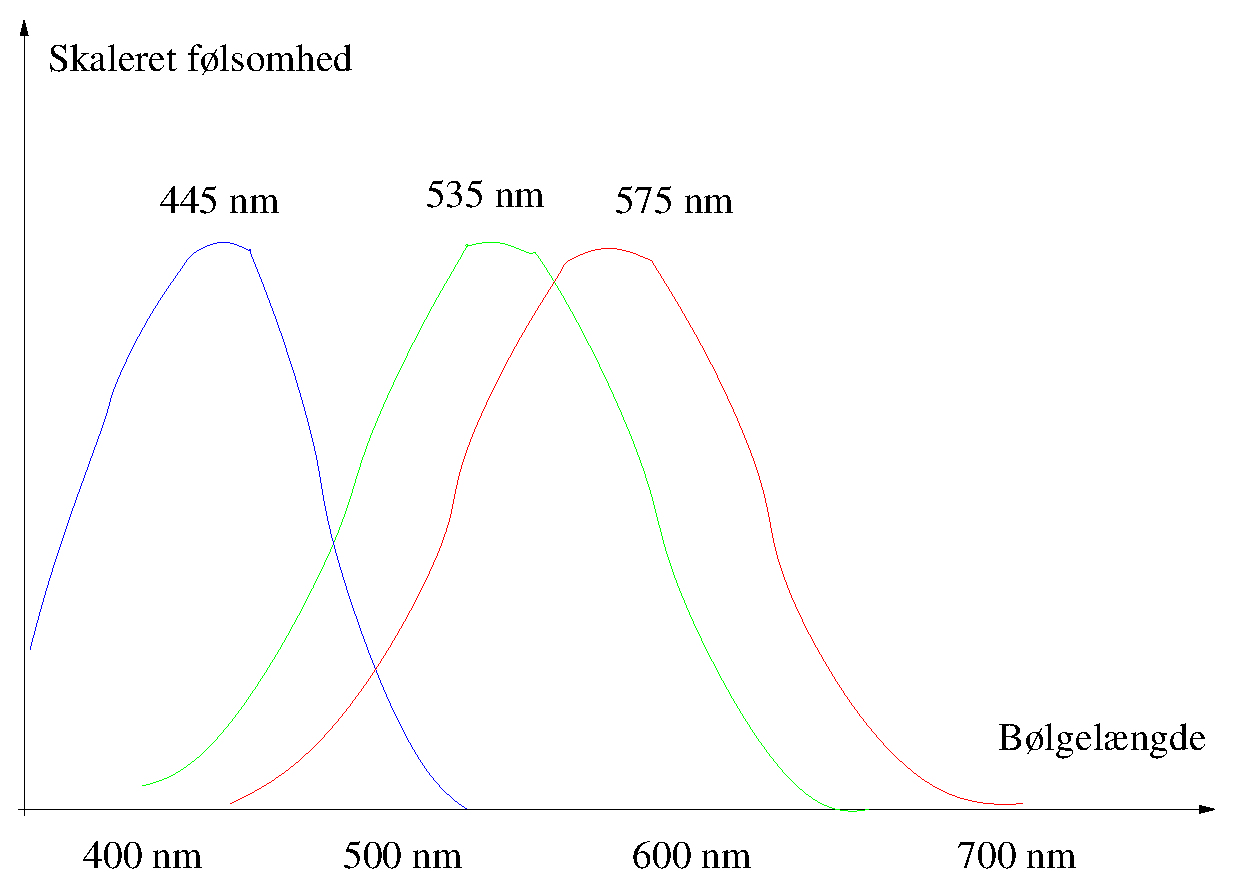
\includegraphics[width=4.5cm]{FIGURE/humaneye.eps}
\end{tabular}
\end{center}
\vspace{3mm}

In the human retina the exist 3 types of conical shaped cells
containing pigment making them sensitive to light within a broad band
of vawelengths.
\end{frame}



%-------------------------------------------------------------------
\begin{frame} 
\begin{itemize}
  \item The digital filters used in a different cameras etc.\ are
        different. The registered RGB-value depends on the sensor. \\[3mm]
  \item The registered RGB-value depends on the spectral distribution of
        the light source $L(\lambda)$, the reflection from the object
        $RF(\lambda)$, and the sensor sensitivity curves $f_{r/g/b}(\lambda)$.
\end{itemize}

{\small
\begin{eqnarray*}
        R & = & k_r \sum_{\lambda} L(\lambda) RF(\lambda) f_r(\lambda) \\
        G & = & k_g \sum_{\lambda} L(\lambda) RF(\lambda) f_g(\lambda) \\
        B & = & k_b \sum_{\lambda} L(\lambda) RF(\lambda) f_b(\lambda) 
\end{eqnarray*}
}
\end{frame}





%-------------------------------------------------------------------
\begin{frame} 
\frametitle{Eksample}

$$
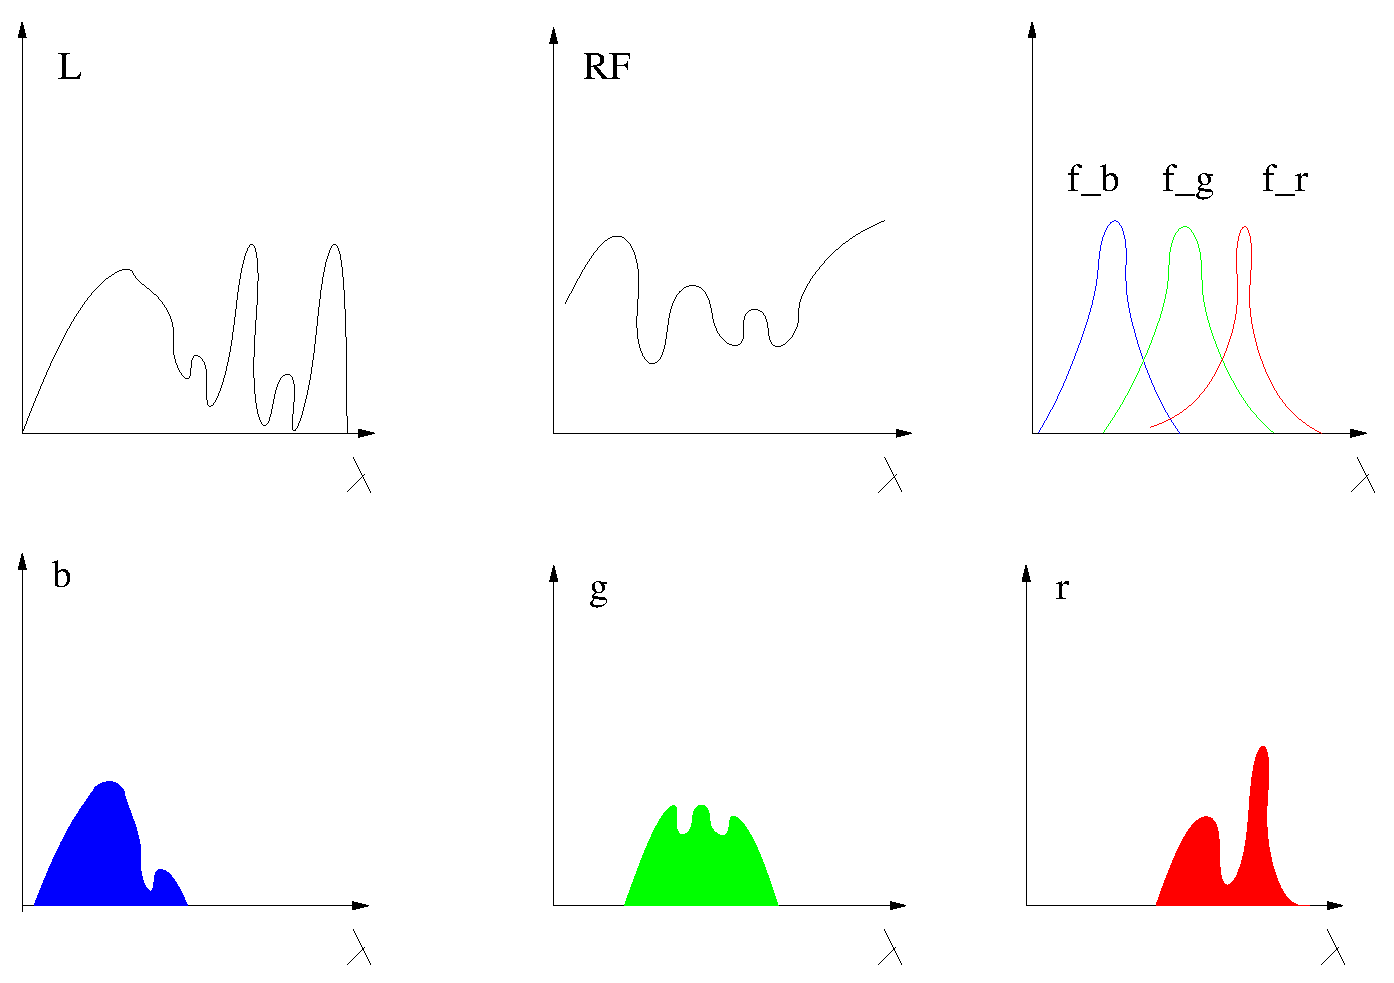
\includegraphics[width=7.8cm]{FIGURE/spectralEX.eps}
$$
\end{frame}



%-------------------------------------------------------------------
\begin{frame}
  \frametitle{Colors in CBIR}
  \begin{itemize}
  \item In CBIR colors could be important \\[3mm]
  \item There are a number of color-extentions to SIFT, including
    opponent-SIFT \\
    $$
       O_1 = \frac{R-G}{\sqrt 2}\;, \hspace{5mm}
       O_2 = \frac{R+G - 2B}{\sqrt 6}
    $$
  \item One approach is to apply color histograms. \\[3mm]
    To compare the histograms they should be quantized equally,
    e.g. into 8 or 12 bins.  Compared to the SIFT-histogram layout
    less histograms (e.g. only one) should be used. \\[3mm]
  \item Hue has been shown to be a good color feature.
  \end{itemize}
\end{frame}




%-------------------------------------------------------------------
\begin{frame} 
\frametitle{HSV}

\begin{tabular}{l l}
  \begin{minipage}[t]{40mm}
  $$
     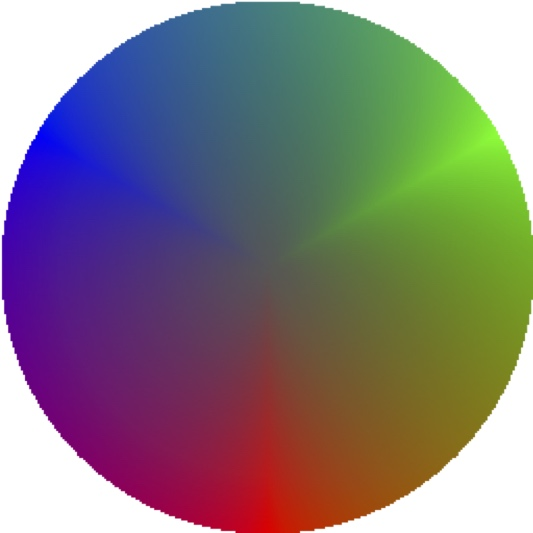
\includegraphics[width=40mm]{FIGURE/Cim.jpg}
  $$
  \end{minipage}
  &
  \begin{minipage}[t]{40mm}
  \vspace{-10mm}
  $$
     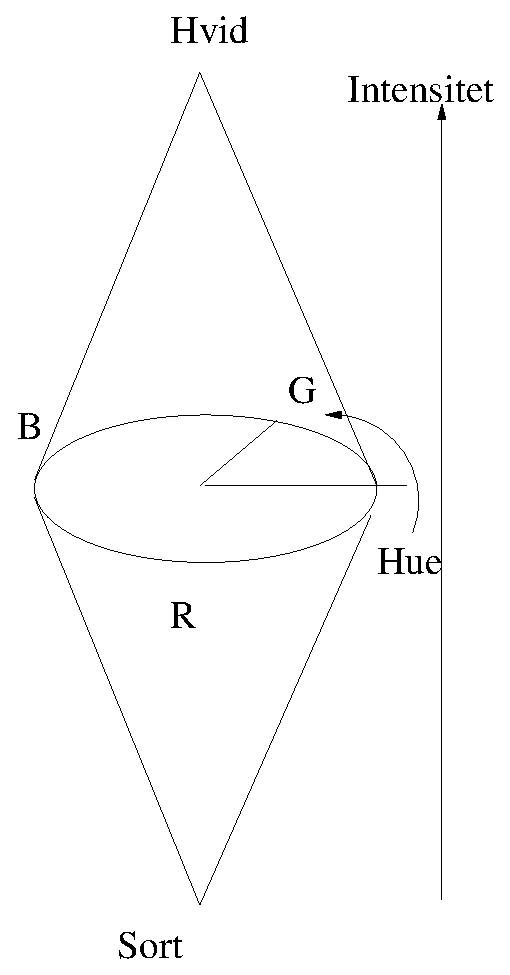
\includegraphics[width=40mm]{FIGURE/hsvfig.eps}
  $$
  \end{minipage}
\end{tabular}
\end{frame}



%-------------------------------------------------------------------
\begin{frame} 
\frametitle{RGB2HSV}
Lad
\begin{displaymath}
 \theta \;=\; \tan^{-1} \left \{
     \frac{2R - G - B}
         {\sqrt{3} (G-B)}
\right \}
\end{displaymath}
 {\color{red}{Hue}} H is definered by:
\begin{displaymath}
 H \;=\; \left \{
      \begin{array}{l l}
           \theta & \mbox{if B $\leq$ G} \\
           360 - \theta & \mbox{if B > G}
       \end{array} \right.
\end{displaymath}
{\color{red}{Intensity}}: $I = \frac{1}{3}( R + G + B)$ og
{\color{red}{Saturation}} S:
\begin{displaymath}
  S \;=\; 1 \;-\; \frac{3}{R + G + B} 
         \left [ \min \left \{ R, G, B \right \} \right ]
\end{displaymath}
Notice the discontinuity of Hue at 0.

\end{frame}



%-------------------------------------------------------------------
\begin{frame}
  \frametitle{Learning the Visual Words: Training}
  \begin{itemize}
  \item Collect all descriptor vectors from a training set of images 
    showing one class. They must have something in common. \\[4mm]
  \item Group descriptors by similarity: clustering. \\[4mm]
  \item Choose prototypical representatives of each cluster: the \textbf{visual words}. \\[4mm]
  \item The set of visual words obtained is called \textbf{vocabulary} or \textbf{codebook}.
  \end{itemize}
\end{frame}


%\subsection{Clustering}
%\label{sec:clust}

%-------------------------------------------------------------------
\begin{frame}
  \frametitle{Clustering}
  \begin{definition}
    (from Wikipedia) Cluster analysis or clustering is the task of
    assigning a set of objects into groups (called clusters) so that
    the objects in the same cluster are more similar (in some sense
    or another) to each other than to those in other clusters.
  \end{definition}
  
  \vfill
  \begin{itemize}
  \item
    I will describe one standard technique for vector clustering: $K$-means clustering.
  \end{itemize}
\end{frame}


%-------------------------------------------------------------------
\begin{frame}
\frametitle{Good clustering}
{\color{red}{Exercise:}} \\
Discuss 2 minutes with your neighbor: What characterizes a good
clustering \\[5mm]
\pause

\begin{itemize}
  \item Small intra-cluster distances 
  \item Large inter-cluster distances 
\end{itemize}
\bigskip

Central for clustering is to have a good distance measure
\end{frame}


%-------------------------------------------------------------------
\begin{frame}
  \frametitle{A 2D Example}
  \begin{itemize}
  \item We want to cluster the following data
    \begin{center}
      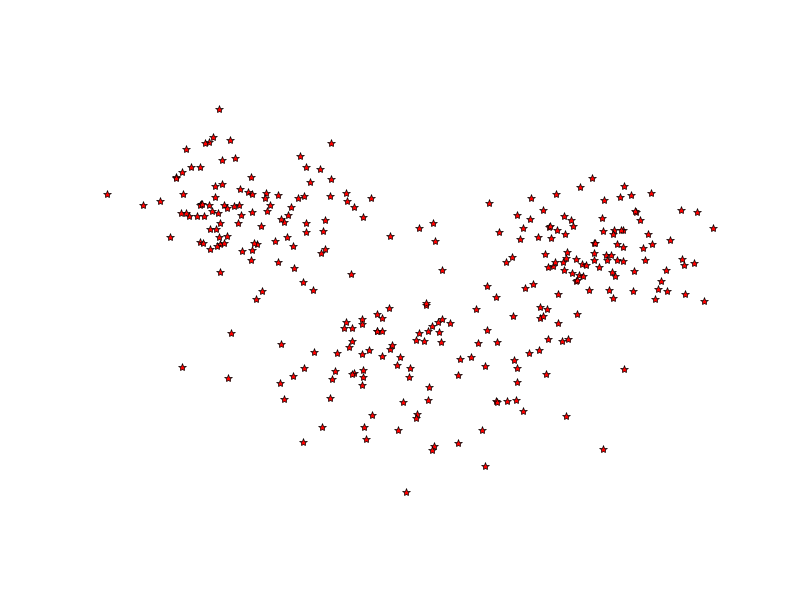
\includegraphics[width=0.8\textwidth]{FIGURE/2DData}
    \end{center}
  \item Visually 3 clusters.
  \end{itemize}
\end{frame}


%-------------------------------------------------------------------
\begin{frame}
  \frametitle{$K$-means Clustering}
  \begin{itemize}
  \item
    Given $n$ data vectors $x_1,\dots,x_n$ in $\RR^d$, find a
    \emph{partition} $\Ss$ of $\{1,\dots,n\}$ into $K$ subsets
    $S_1,\dots,S_K$, such that the \emph{Distortion} $\Dd$
    $$
    \Dd(S_1,\dots,S_K) = \sum_{i = 1}^K\sum_{j\in S_i} \|x_j -\mu_i\|^2
    $$
    is minimum, with
    $$
    \mu_i = \frac{1}{\#S_i}\sum_{j\in S_i}x_m = \text{mean of the }x_j, j\in S_i.
    $$
  \item The means $\mu_i$ become the prototypical representatives of
    the vectors, i.e., \textbf{the words} 
  \end{itemize}
\end{frame}


%-------------------------------------------------------------------
\begin{frame}
  \frametitle{Standard Algorithm (Lloyd's Algorithm)}
  \begin{itemize}
  \item Choose  $K$ candidate cluster means $m_1,\dots,m_K$ (randomly).\vfill
  \item Then iterates the following two steps until no significant change occurs in the distortion $\Dd$\vfill
    \begin{enumerate}
    \item Assignment step: assign each observation $x_j$ to the cluster with closest mean $m_i$\vfill
    \item Update step: recompute the means of the clusters.\vfill
    \end{enumerate}
  \item {\color{red}{Exercise:}} Discuss for one minute with your
      neighbor: Does K-means always converge ?
  \end{itemize}
\end{frame}


%-------------------------------------------------------------------
\begin{frame}
  \begin{itemize}
   \item K-means always converge, but not necessarily fast nor to the
     right clustering. \\[4mm]
  \item To avoid local minima, run the {\em k-means} with different
    initial candidate clusters og choose the best, i.e.\ the one with
    minimal \emph{Distortion} $\Dd$. \\[4mm]
  \item The \emph{Distortion} $\Dd$ is specified by the sum of distances from
    each point to the nearest cluster (but there are other approaches). \\[4mm]
  \item You have to fix $K$.  There is no easy way to choose the
    optimal value. 
  \end{itemize}
\end{frame}


%-------------------------------------------------------------------
\begin{frame}
  \frametitle{2D example, $K = 3$}
  \begin{itemize}
  \item Run of $K$-means on the previous data.
    \begin{center}
      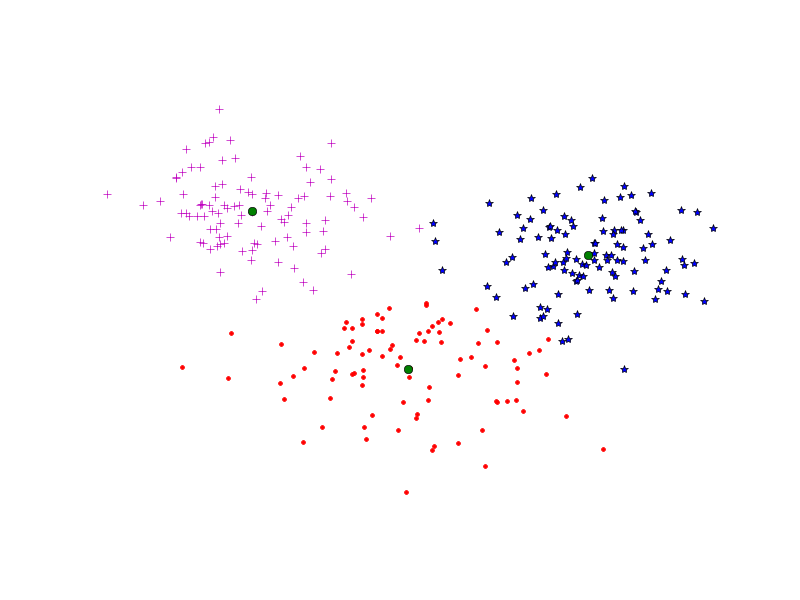
\includegraphics[width=0.8\textwidth]{FIGURE/2DData3Clusters}
    \end{center}
  \end{itemize}
\end{frame}


%-------------------------------------------------------------------
\begin{frame}
  \begin{itemize}
  \item Run with $K = 2$.
    \begin{center}
      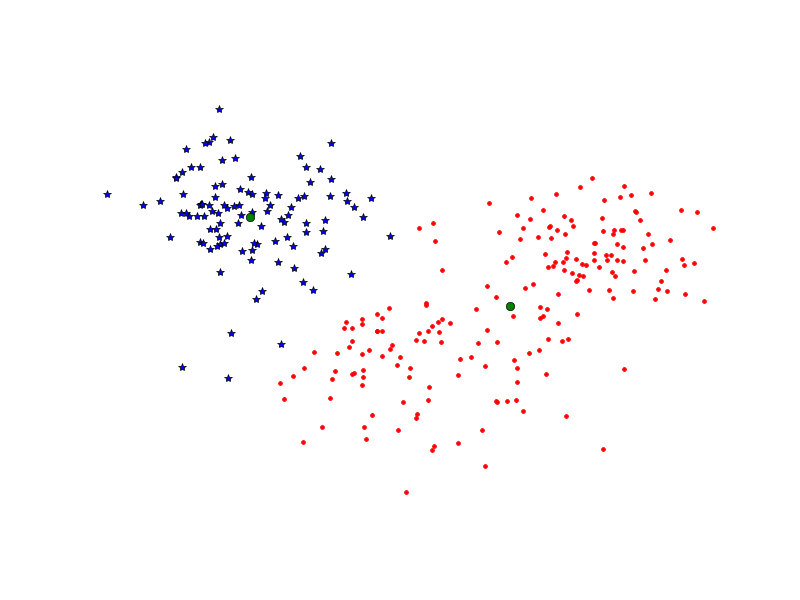
\includegraphics[width=0.8\textwidth]{FIGURE/2DData2Clusters}
    \end{center}
  \item $K$ can have a deep impact in the clustering results. 
  \end{itemize}
\end{frame}




%-------------------------------------------------------------------
\begin{frame}
\frametitle{Which K ?}
  \begin{itemize}
    \item Most algorithms for clustering assumes K known \\[2mm]
    \item For very low-dimensional data visual exploration techniques
      (eg. plot3($\cdot$) in Matlab) may be used to guess K \\[2mm]
    \item For high-dimensional data an optimal choice is difficult to
      guess \\[2mm]
    \item K too small $\Longrightarrow$ Cannot model data \\[2mm]
    \item K too large $\Longrightarrow$ Overfitting \\[2mm]
    \item Problem: Often the average training error decreases 
      smoothly with K (no sudden decrease)
    \item For CBIR, K should be counted in thousands, and an accurate
      optimal choice is neither needed nor easy to find.
  \end{itemize}
\end{frame}




%-------------------------------------------------------------------
\begin{frame}
  \frametitle{Other Clustering Methods}
  \begin{itemize}
  \item {\em Minimum Spanning tree}: Connect all points to its closest
    neighbor. Then iteratively remove the longest edge until left with
    $K$ clusters. \\[3mm]
  \item Hierarchical clustering: group data points by proximity,
    creates a binary tree-structure.  Each non-leaf node contains
    average distance between it subtrees. Clustering is performed by
    distance threshold. Number of clusters is not predefined. \\[3mm]
  \item Distribution model: observed data is produced by $K$
    distributions: clusters belong most likely to the same
    distribution, EM - {\em Expectation - Maximization}
    Algorithms. Can be very powerful. 
  \end{itemize}
\end{frame}


%-------------------------------------------------------------------
\begin{frame}
  \frametitle{Clustering and Words}
  \begin{center}
    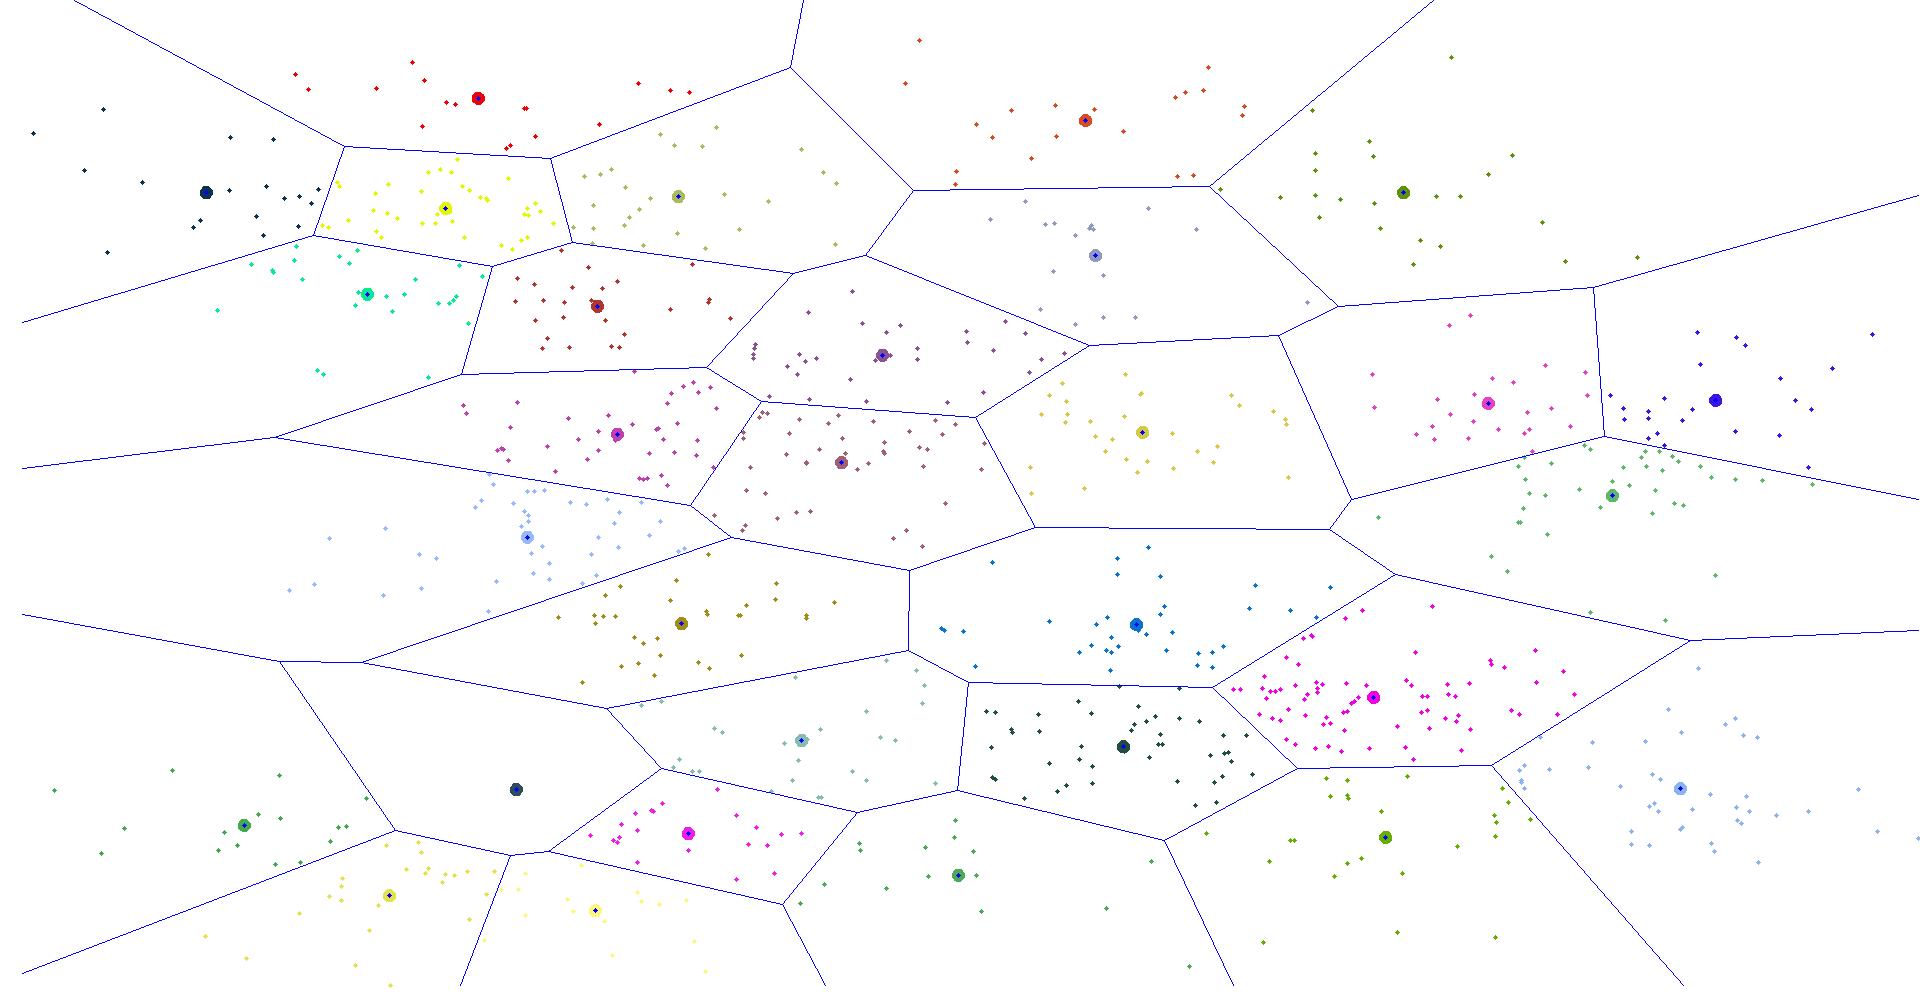
\includegraphics[width=0.6\textwidth, height=0.58\textheight]{FIGURE/clustervoronoi}
  \end{center}
  \begin{itemize}
  \item Words are cluster centers
  \item Each observation is assigned to the Voronoi cell it belongs to.
  \end{itemize}
\end{frame}


%-------------------------------------------------------------------
\begin{frame}
  \frametitle{Bag of Visual Words Representation of Images}
  \begin{itemize}
  \item Once the vocabulary is obtained, each image is ``projected'' to the vocabulary:
    \begin{enumerate}
    \item Compute descriptors for the image,
    \item Assign each of them to its closest word
    \item Count the number of occurrences of each word in the image. i.e.
      compute the histogram of the words for this image. 
    \end{enumerate}
  \item This histogram is the \textbf{Bag of words} (BOW) representation of
    the image.
  \item Spatial arrangement of the words is forgotten. Words are just ``thrown in a bag''.
  \item Histograms can be normalized. Each entry becomes the
    \textbf{word frequency} (or \textbf{term frequency}) in the image.
  \end{itemize}
\end{frame}


%-------------------------------------------------------------------
\begin{frame}
\frametitle{When do BOW malfunction}

{\color{red}{Exercise:}} \\
Discuss 2 minutes with your neighbor when a Bag of Words
representation is insufficient or misleading \\[4mm]
\pause

Example: When spatial arrangement do matter, eg. ``Putin on Obama''.
\pause
    \begin{center}
      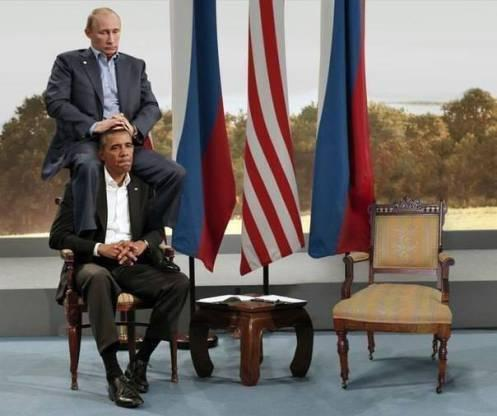
\includegraphics[width=0.5\textwidth]{MyImages/PutinOnObama.jpg}
    \end{center}
\end{frame}



% \section{Similarity Measures}
% \label{sec:simmeas}


%-------------------------------------------------------------------
\begin{frame}
  \frametitle{Ensemble of Common Words}
  \begin{itemize}
  \item Simple similarity measure: count the amount of common words between images \\[4mm]
  \item Can be used for query: return the images that have these ``words'' in common. \\[4mm]
  \item A subset of words can be used. %\\[3mm]
%   \item Easy to implement within a standard relational database. \\[3mm]
%   \item Discard bin sizes in histograms.
  \end{itemize}
\end{frame}


%-------------------------------------------------------------------
\begin{frame}
  \frametitle{Euclidean and Histogram Distances for BoVW}
  \begin{itemize}
  \item Euclidean Distance between two vectors 
    $$
    v_1 = \left(v_{11},\dots,v_{2K}\right), v_2 = \left(v_{21},\dots,v_{2K}\right), 
    d(v_1,v_2) = \sqrt{\sum_{i=1}^K\left(v_{1i}-v_{2i}\right)^2}
    $$
  \item Bhattacharyya Distance for Normalized Histograms:
    $$
    d(v_1,v_2) = \sum_{i=1}^K\sqrt{ v_{1i}\, v_{2i}}
    $$
  \item Kullback-Leibler Divergence for Normalized Histograms
    $$
    D_{KL}(v_1||v_2) = \sum_{i=1}^Kv_{1i}\,\ln\frac{v_{1i}}{v_{2i}}
    $$
    Not a distance as not symmetric, but can be symmetrized 
    $$
    d_{KL}\left(v_1,v_2\right) = \frac12\left( D_{KL}(v_1||v_2) +  D_{KL}(v_2||v_1)\right)
    $$
  \item $\chi^2$-distance measure $\sum \frac{|v_{1i} - v_{2i}|}{|v_{1i} + v_{2i}|}$
  \item {\em Earth movers distance}
  \end{itemize}
\end{frame}


%-------------------------------------------------------------------
\begin{frame}
  \frametitle{The Term Frequency -- Inverse Document Frequency }
  \begin{itemize}
  \item Some words (terms) are more common than other, not in one
    document but in a \textbf{corpus} (or data set). \\[3mm]
  \item Such terms are in general \textbf{less informative} \\[3mm]
   % (might be seen as a tautological statement!) 
  \item {\color{red}{Inverse Document Frequency}} $idf$ weighting
    reduces their importance:  For a given word $w$ and a corpus $D$ \\[3mm]
    $$
    \idf_w = \frac{\mbox{Number of documents or images}}{\mbox{number
        of document in wich w appears}} 
    $$
    $\idf_w$ is a global weight for the word $w$.

  \end{itemize}
\end{frame}


%-------------------------------------------------------------------
\begin{frame}
  \begin{itemize}
  \item Sometimes the logarithm of the fraction above is used
    $$
    \idf_w = \log \left (\frac{\mbox{Number of documents orimages}}{\mbox{number
        of document in wich w appears}} \right )
    $$
  \item The \textbf{tf-idf} approach reweights the normalized histogram
    entries of document $d$ (the term frequencies) by the $idf$'s. \\[2mm]
    \textbf{tf-idf} = \textbf{$\idf_w \times $} \textbf{tf} \\[3mm]
  \item Alternatively the Euclidean Distance or angle used as similarity. For a document
      $d$ in the data set and a query document $q$ 
      Compute the tf-idf reweighted BoW's $v_d$ and $v_q$. 
    \item Define the similarity
      $$
         \text{sim}(d,q) = \text{angle}(v_d,v_q) = \arccos\frac{v_d\cdot v_q}{\|v_d\|\|v_q\|}
      $$
    \item In practice, the arc cosine is not computed. sim$(d,q)$ is the
      range [0,1], maximum similarity is 1. 
  \end{itemize}
\end{frame}


% \section{Conclusion}


%-------------------------------------------------------------------
\begin{frame}
  \frametitle{Conclusion}
  \begin{itemize}
  \item We have been through the major steps for a Content-Based Image Retrieval
    System based on the notion of learned vocabulary and bag of visual
    words.
  \item Selection interest point detectors and descriptors 
  \item Step of training -- learning vocabulary using clustering
  \item Step of Indexing -- computing visual words and histograms
    (BoW's) of visual words
  \item Tools for searching / ranking -- computing similarity measures.
  \item Bag of Words is also used for object classification and recognition.
  \item Main limitation is that BoW ignores spatial relationships among the words
  \item Incorporating them is a hot research topic.
  \end{itemize}
\end{frame}

%-------------------------------------------------------------------
\begin{frame}
  \frametitle{Successful query?}
  \begin{center}
    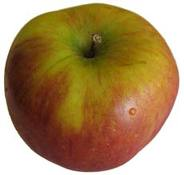
\includegraphics[width=0.2\textwidth]{FIGURE/anapple}\\
    
\includegraphics[width=0.05\textwidth]{FIGURE/redarrow}\\
    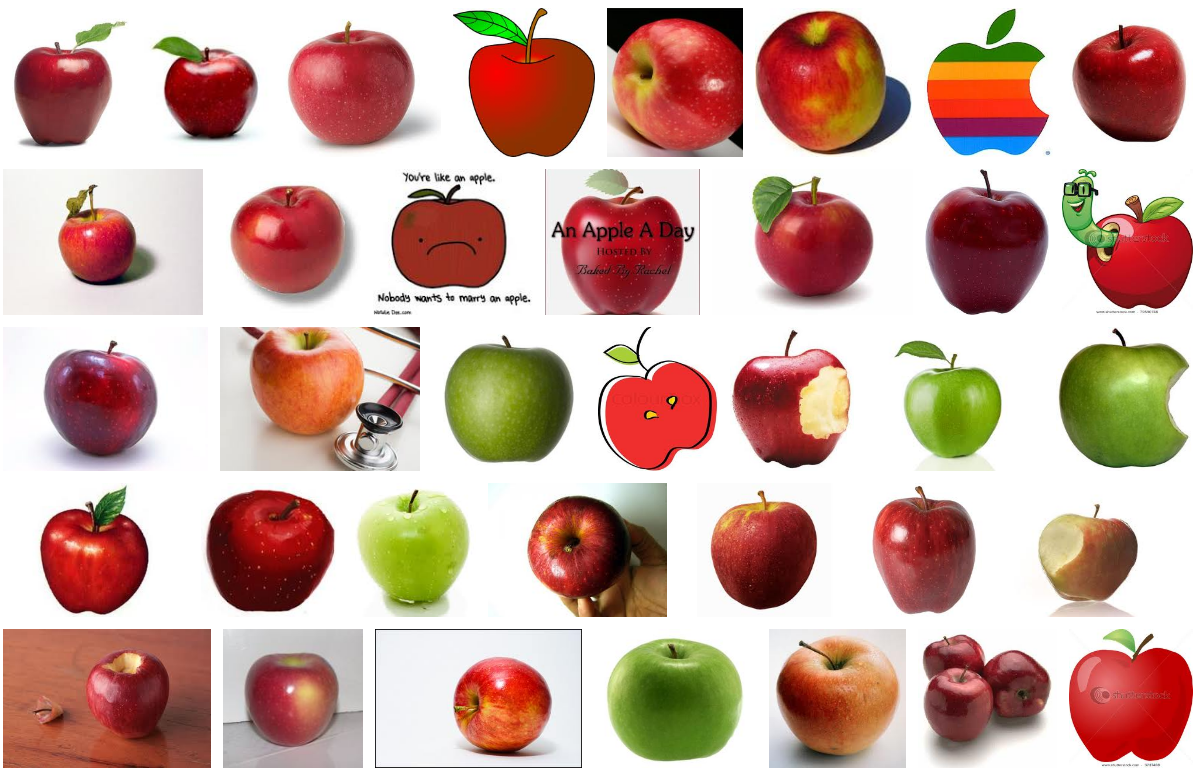
\includegraphics[width=0.6\textwidth]{FIGURE/applequery}\\
  \end{center}
\end{frame}


% \begin{frame}
%   \frametitle{A really smart CBIR system?}
%   \begin{center}
%    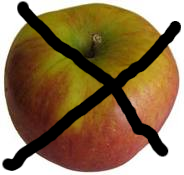
\includegraphics[width=0.2\textwidth]{FIGURE/noapple}\\
%    
\includegraphics[width=0.05\textwidth]{FIGURE/redarrow}\\
%    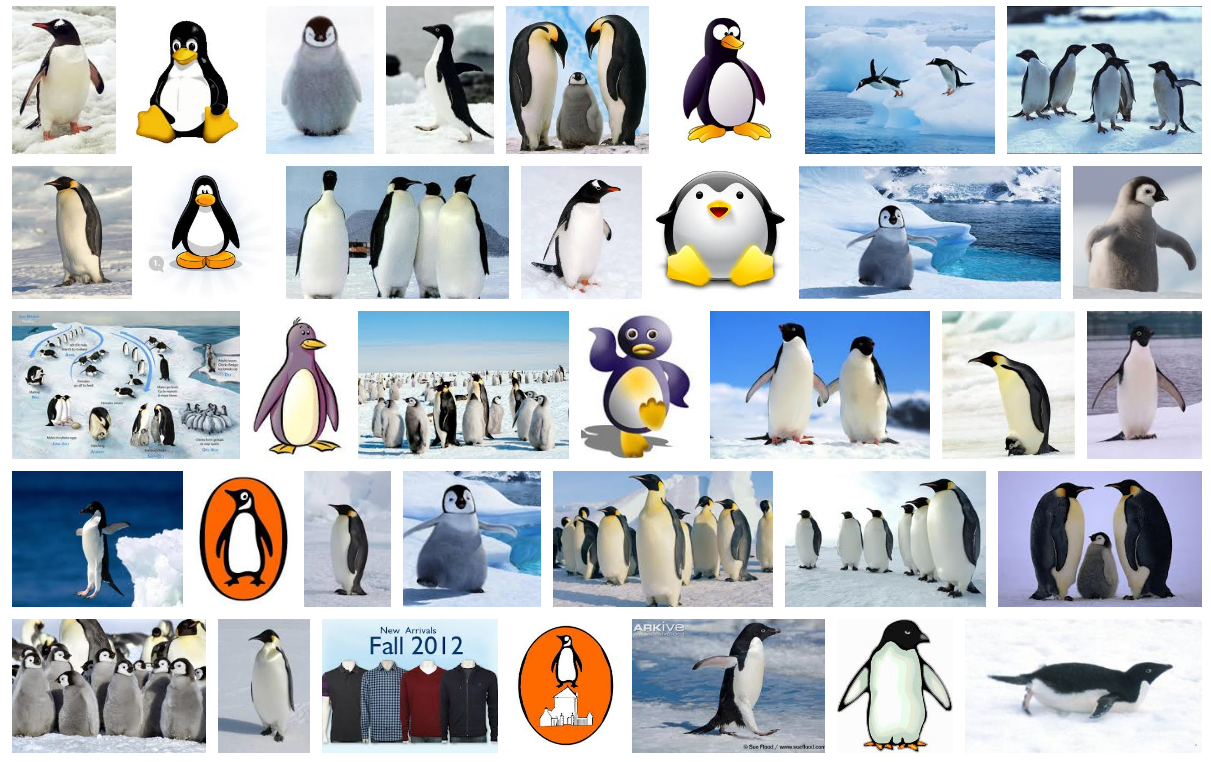
\includegraphics[width=0.6\textwidth]{FIGURE/Penguins}\\
%   \end{center}
% \end{frame}



%-------------------------------------------------------------------
% \begin{frame}
%  \frametitle{Assignment - details}
%  \begin{itemize}
%  \item The assignment consists in implementing a prototypical Content
%    Based Image Retrieval System \\[5mm]
%  \item Four parts:
%    \begin{enumerate}
%      \item Gather descriptors in training image data set \\[3mm]
%      \item Construct codebook using k-means and Bag-Of-Words \\[3mm]
%      \item Project test images onto codebook, and generate BoW \\[3mm]
%      \item Retrieve according to similarity measure
%    \end{enumerate}
%  \end{itemize}
% \end{frame}

%-------------------------------------------------------------------
% \begin{frame}
% \frametitle{What descriptors}
%  \begin{itemize}
%     \item   You are advised to use SIFT features
%     \item   Few versions of SIFT include color. You may miss a lot of
%       information. 
%     \item   Color histograms etc.
%     \item   Other descriptors: Texture
%     \item   Advise: Keep it simple
%  \end{itemize}
% \end{frame}

%-------------------------------------------------------------------
% \begin{frame}
%   \frametitle{Training and testing}
%   \begin{itemize}
%    \item Split data into two parts. Don't look at the test data before
%      testing \\[5mm]
%    \item During development you may split the training data into a
%      construction part and an evaluation part \\[5mm]
%    \item Never use the test set for tuning ! \\[5mm]
%    \item Download Caltech-101 image database (131 MB) with 101
%      categories or the newer Caltech-256 base (1.2 GB)
%  \end{itemize}
% \end{frame}


%-------------------------------------------------------------------
% \begin{frame}
%  \frametitle{Data enough?}
%  \begin{itemize}
%    % \item One SIFT-key takes $2^{7+2}$ bytes. 
%    \item Say we use 1000 clusters and need about 1000  
%      elements per cluster, in total about 1M features for training. \\[3mm]
%    \item The image size (of Caltech-101) is about $200 \times 300$
%      generating on average about 1 percent key points [decriptors],
%      say 1000. \\[3mm]  
%%    \item To reach the needed amount af data for training we need at
%%      least 1000 images (in practice more).
%    \item The Calatech 101 base  has 101 categories with 40-800
%      images/category, in total  9450 images.\\[3mm]
%    \item {\color{red}{Exercise: Discuss with your neighbor: How many
%          images/category can you save for testing ?}}
%  \end{itemize}
% \end{frame}

%-------------------------------------------------------------------
% \begin{frame}
% \frametitle{What then?}
%  \begin{itemize}
%    \item {\color{red}{Exercise: Discuss with your neighbor: How many
%          images/category can you save for testing ?}} \\[3mm]
%    \pause
%      On average, 9450 images provides about 10M SIFT-descriptors. We need 
%      1M for training leaving 9M (or 90\%) for testing. We have plenty
%      of data. \\[3mm]
%    \item {\color{red}{What if we only have 20 images in one category
%          and these images only generate 500 decriptors each ?}} \\[3mm]
%      \pause
%      Difficult to say, because we don't know if the images would
%      generate new clusters. \\
%    \item In general, we often want more data to make sure that it
%      spans the complete range of possibilities.  
%  \end{itemize}
% \end{frame}




%-------------------------------------------------------------------
% \begin{frame}
%  \frametitle{What error ?}
%  \begin{itemize}
%    \item Error on training data versus error on test data \\[5mm]
%    \item {\color{red}{Exercise: Explain what is the problem when
%      the training error is less than the test error? }} \\[5mm]
%    \pause
%    \item Overfitting is a serious problem.  Often caused by using too
%      few training data (or too complicated model) \\[5mm]
%    \item We want to generalize in order to retrieve/classify new data
%  \end{itemize}
% \end{frame}


%-------------------------------------------------------------------
% \begin{frame}
%  \frametitle{Cross-validation}
%  \begin{itemize}
%    \item Divide data into say 10 sets (10-fold CV) \\[5mm]
%    \item Train on all but one set that is used testing \\[5mm]
%    \item Retrain and test on all possible combinations \\[5mm]
%    \item Compute the average test error
%  \end{itemize}
% \end{frame}


%-------------------------------------------------------------------
% \begin{frame}
%   \frametitle{How to report}
%  \begin{itemize}
%    \item Amount: 8 pages including everything: 
%      Try to be concise, structured etc. Keep text less than 2-3 pages \\[5mm]
%    \item Discussion: This is the most important part \\[5mm]
%    \item Tables: Remember to tell me what I should notice \\[5mm]
%    \item Figures: Remember axis labels etc.  What should I see? \\[5mm]
%    \item Images: Don't show them too small. What should I see? \\[5mm]
%    \item Explanations: Don't expect me to guess what you mean or see yourself
%  \end{itemize}
% \end{frame}


%-------------------------------------------------------------------
% \begin{frame}
%%   \frametitle{Questions}
%    $\mbox{}$ \\[16mm]
% 
% \begin{center}
%   {\Huge {\color{blue}{QUESTIONS}}}
% \end{center}
% \end{frame}



\end{document}
